\chapter{Introduction}

\section{Research Background and Motivation}

Understanding spatial openness in residential housing is fundamental to enhancing living quality and guiding 
architectural design practices. In urban environments, particularly in densely populated cities like Tokyo, the 
perception of spatial openness significantly impacts residents' psychological well-being, comfort, and overall 
satisfaction with their living spaces. Traditional architectural evaluation methods have long relied on basic 
quantitative metrics such as floor area, room count, and ceiling height to assess spatial quality. However, these 
conventional indicators fail to capture the nuanced spatial qualities that contribute to the subjective experience 
of openness in residential environments.

The concept of spatial openness extends beyond mere physical dimensions to encompass the complex interplay between 
visual connectivity, visibility of interior elements, and so on. In the context of rental housing markets, where 
prospective tenants make decisions based on limited visual information from online platforms, understanding how 
spatial openness translates through digital representations becomes increasingly important. The proliferation of 
online rental platforms has created unprecedented opportunities to analyze large-scale housing data, including 
interior imagery and floor plans, which can provide insights into spatial characteristics that were previously 
difficult to quantify systematically.

Tokyo's 23 special wards represent a unique data playground for studying spatial openness due to the city's 
distinctive urban morphology, diverse architectural styles spanning multiple decades, and the comprehensive 
digitization of rental housing information, which has always been one of the most populared cities and rental 
market in the world.

\section{Literature Review and Research Gaps}

\subsection{Spatial Openness in Recent Architectural Research}

The study of spatial openness has been approached from various perspectives within architectural and environmental 
psychology research. Traditional spatial analysis methods have focused on geometric properties and numerical metrics 
of building attributes. Space syntax theory, developed by Hillier and Hanson, introduced systematic approaches to 
understanding spatial relationships through graph-based analysis of architectural layouts \cite{hillier1987ideas}. 
Visibility Graph Analysis (VGA), as an extension of space syntax principles, provides a quantitative framework for 
measuring visual connectivity and spatial integration within architectural spaces.

Recent research has expanded the understanding of spatial openness to encompass cultural and contextual dimensions. 
AL-Mohannadi et al. demonstrated how spatial configurations in traditional Qatari domestic architecture embody 
cultural values of privacy and openness through sophisticated spatial arrangements, highlighting the importance of 
considering cultural context in spatial analysis \cite{almohannadi2020cultural}. This perspective emphasizes that 
spatial openness is not merely a physical property but a culturally-mediated experience that varies across different 
architectural traditions.

The methodological approaches to analyzing spatial configurations have also evolved significantly. Kim and Choi 
introduced Angular VGA and Cellular VGA as innovative extensions of traditional space syntax methods, providing 
more nuanced ways to analyze human movement behavior in architectural spaces \cite{kim2009angular}. These 
methodological advances enable researchers to capture the dynamic aspects of spatial experience that conventional 
VGA might overlook. Furthermore, recent work by Jahan et al. on wheelchair users' navigation challenges has 
highlighted the importance of considering diverse mobility perspectives when evaluating spatial accessibility 
and openness in urban environments \cite{jin2024spatial}. Their framework for "dynamic walkability" underscores 
how spatial openness must accommodate various user needs and movement capabilities.

The abovementioned previous researches have demonstrated that spatial openness influences occupant behavior, movement patterns, and 
psychological responses to built environments. Studies in environmental psychology have shown that perceived openness 
correlates with reduced stress levels, improved cognitive performance, and enhanced overall well-being. However, most 
existing research has been limited to small-scale case studies or controlled experimental settings, lacking the scale 
and diversity necessary to understand spatial openness patterns across entire urban regions.

\subsection{Computer Vision and Spatial Analysis}

Recent advances in computer vision and deep learning have opened new possibilities for automated spatial analysis. 
Semantic segmentation techniques enable the extraction of architectural elements from images, allowing for systematic 
analysis of interior compositions. Similarly, these deep-learning-based models have been successfully applied to recognize and 
classify various architectural features in floor plans, including walls, windows, floors, and ceilings. These technological 
developments create opportunities to process large-scale image datasets that would be impractical to analyze manually.

The integration of 2D image analysis with 3D spatial analysis recently draws more attentions in architectural research. While 
2D analysis can capture visual qualities and material compositions, 3D analysis provides insights into spatial 
relationships and configurational properties. The combination of these approaches offers a more comprehensive 
understanding of spatial openness than either method alone.

\subsection{Big Data Opportunities and Research Gaps}

The emergence of big data analytics in housing research has revealed new patterns in residential preferences, market 
dynamics, and architectural trends. Online rental platforms generate vast amounts of data, including property 
specifications, pricing information, and visual documentation through interior images and floor plans. This data 
richness enables researchers to investigate questions about spatial quality and market valuation at unprecedented 
scales, creating opportunities that were previously impossible due to data limitations.

However, the potential for using big data to understand subjective spatial experiences remains largely unexplored, 
particularly in the context of rental housing markets that traditionally rely on rule-based tabular data without 
in-depth understanding of spatial qualities. While studies using conventional tabular data can achieve large scale, 
spatial openness research involving image analysis or human-operated software assessments has been limited to small 
samples, preventing generalization to broader urban contexts. There have been some explorations in retrieving more 
abstracted representations of data types like floor plans using machine-driven automated approaches \cite{yamada2021graph}, 
but these methods tend to focus on structural representations with limited interpretation abilities due to the format, such as network-style graphs. Additionally, the tools and methodologies for 
systematically processing and analyzing large-scale visual and spatial data in housing research are still developing, creating both opportunities and challenges for comprehensive spatial analysis.

\section{Primary Research Objectives}
This research aims to address the identified gaps through the following primary objectives:

\begin{enumerate}
    \item \textbf{Develop a Comprehensive Methodology}: Create a multifaceted evaluation method for spatial openness 
    that combines automated extraction of visual elements from interior images with floorplan semantic segmentation 
    for VGA simulations, enabling large-scale analysis previously limited by manual assessment constraints.
    
    \item \textbf{Large-Scale Analysis}: Conduct systematic analysis of spatial openness using large-scale rental 
    housing data from Tokyo's 23 wards.
    
    \item \textbf{Temporal and Geographic Investigation}: Examine how spatial openness varies across construction 
    periods and geographic regions within Tokyo's 23 wards.

    \item \textbf{Feature Dependency Analysis}: Investigate relationships between 2D visual elements and 3D spatial 
    connectivity measures to identify key interactions contributing to spatial openness perception.

    \item \textbf{Market Correlation Analysis}: Explore the relationships between spatial openness features, impression evaluations and rental 
    costs.
\end{enumerate}


\section{Structure of the Thesis}

This thesis is organized into six main chapters, each addressing specific aspects of spatial openness analysis:

\textbf{Chapter 1: Introduction} provides the research background, literature review, objectives, and methodology 
overview.

\textbf{Chapter 2: Methodology} presents detailed descriptions of the Lifull dataset, openness quantification methods 
including interior image-based 3D perceptionanalysis and floor plan-based 2D VGA analysis, and statistical analysis frameworks.

\textbf{Chapter 3: Results} presents the primary findings, including temporal analysis of openness characteristics 
across construction decades and geographic distribution analysis across Tokyo's 23 wards.

\textbf{Chapter 4: Conclusions} summarizes key findings and outlines future research directions.


The thesis concludes with comprehensive appendices containing detailed technical specifications, additional statistical 
analyses, and supplementary materials that support the main findings.

Figure \ref{fig:method_flow} illustrates the overall framework used in this study, showing the integration of various data sources and analytical approaches to quantify spatial openness.

\begin{figure}[htbp]
    \centering
    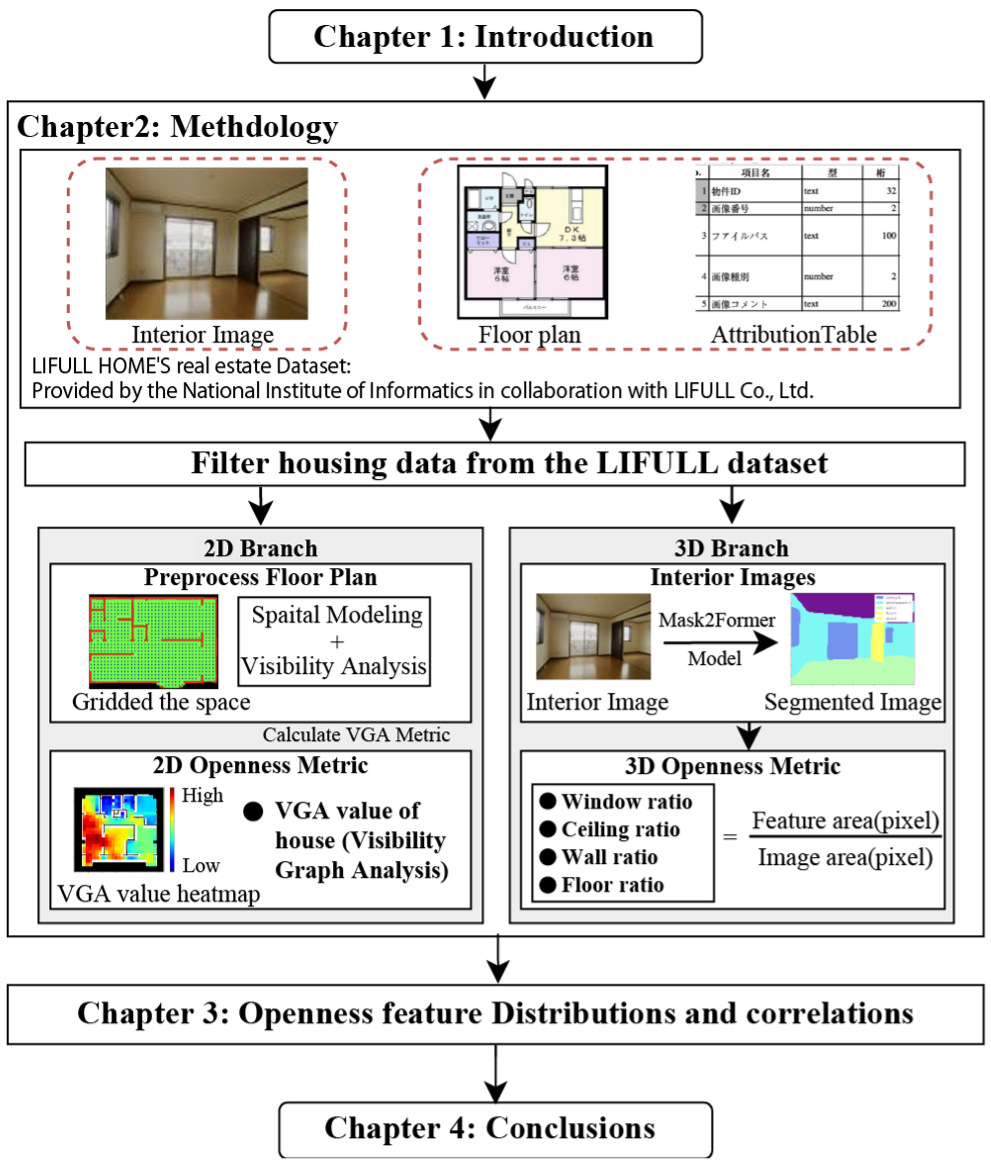
\includegraphics[width=0.8\textwidth]{chapters/plots/method_flow.png}
    \caption{Overall framework showing the integration of various data sources and analytical approaches to quantify spatial openness}
    \label{fig:method_flow}
\end{figure}